\chapter{Trees, branches and (square) roots: why evolutionary relatedness is not linearly related to functional distance}
\chaptermark{Trees, branches and (square) roots}

\graphicspath{{Chapter3/Figs/}}

\begin{center}

{\large Andrew D. Letten and William K. Cornwell}

\small\textit{\textbf{Methods in Ecology and Evolution}} \textbf{(2014)}\\
\url{http://doi.wiley.com/10.1111/2041-210X.12237}

\vspace{1in}

\includegraphics[width=0.15\linewidth]{Chapter3/Figs/Einstein_whitejpg}

\vfill
This study was conceived by ADL and WCK. ADL and WCK contributed equally to scripting code for simulations and writing the manuscript. 

\end{center}

\newpage
\section{Summary}

\begin{enumerate}

\item{ 
An increasingly popular practice in community ecology is to use the 
evolutionary distance amongst interacting species as a proxy for their 
overall functional similarity.
}

\item{
At the core of this approach is the  implicit, yet poorly recognized, 
assumption that trait dissimilarity increases linearly with divergence time, 
i.e. all evolutionary time is considered equal. However, given a classic 
Brownian model of trait evolution, we show that the expected functional 
displacement of any two taxa is more appropriately represented as a linear 
function of time's square root. 
}
\item{
In light of this mismatch between theory and methodology, we argue that
current methods at the interface of ecology and evolutionary biology often greatly 
overweight deep time relative to recent time. 
}
\item{
An easy solution to this weighting problem is a square--root transformation of 
the phylogenetic distance matrix. Using simulated models of trait evolution 
and community assembly, we show that this transformation yields considerably 
higher statistical power, with improvements in 92\% of trials. This methodological update is likely to improve our understanding of the connection between evolutionary relatedness and contemporary ecological processes.
}
\end{enumerate}

\newpage

\section{Introduction}

With increasingly precise estimates of the most common ancestor amongst interacting species, modern phylogenetics offers the 
promise of a synthesis of contemporary ecology and evolutionary history \citep{Webb2002, Johnson2007, Cavender-Bares2009, cadotte2013, 
Swenson2013}. Following on this, the last 10-15 years have seen a precipitous rise in the number of studies examining ecological 
patterns and processes through the lens of evolutionary relatedness. Whilst this integrative approach has undoubtedly yielded new 
insights, much of the foregoing research has proved inconclusive; contemporary ecological interactions often appear, using 
conventional methods, to be unrelated to evolutionary history \citep{Cahill2008, Bennett2013, Narwani2013, Fritschie2013}. In this 
comment we offer one explanation for the poor performance of the phylogenetic metrics used in contemporary ecology, as well as a 
partial solution.

From the beginning of the phylogeny--ecology synthesis, evolutionary 
relatedness has often been used a proxy for the traits mediating species' 
interactions with each other and their environment. It is impossible to 
measure all the relevant traits for complex ecological interactions, but 
because evolution is a conservative branching process and traits are on 
average more conserved than random, phylogenies have the potential to provide 
an integrative measure across all traits \citep{Webb2000}. It follows that the 
strength of this inference is contingent on an accurate model of how 
phylogenetic and functional distance covary. There is a widespread assumption in the literature \citep[see Figure 1b of][] 
{cadotte2013} that phylogenetic and functional distance scale linearly.  This assumption is 
implicit in many of the conventional metrics for assessing phylogenetic community structure and 
phylogenetic diversity \citep{vellend2010}. Below we consider this assumption 
critically, using current theory on trait evolution.  

The classic, ``default'' model for trait evolution is Brownian motion 
\citep[Figure \ref{sq_root_fig}b and][]{Felsenstein1985}.
The diffusion equation for Brownian motion \citep{Einstein1905} has the form:
\begin{equation} 
\frac{\partial\rho}{\partial t}=\sigma^2\frac{\partial^2\rho}{\partial x^2}
\end{equation} 

where $\sigma^2$ is the diffusion constant, t is time, $\rho$ is density and $x$ is position in space. That equation has the solution:
\begin{equation} 
\rho(x,t)=\frac{\rho_0}{\sqrt{4\pi \sigma^2t}}e^{-\frac{x^2}{4\sigma^2t}}
\end{equation} 
which implies that the second moment of the distribution is:
\begin{equation} 
\overline{x^2}=2\sigma^2t.
\end{equation} 
In other words, the variance goes up linearly with time and the standard deviation rises with time's square root, or as 
Einstein put it: ``the mean displacement is therefore proportional to the square root of the time''. Applied in a phylogenetic context 
this means that while among species variance in trait values goes up linearly 
with time \citep{Felsenstein1985}, the expected displacement of any two taxa in trait space
does not increase linearly with time, but rather with time's square root (Figure \ref{sq_root_fig}). This non-linearity is true both for one trait
and for Euclidean distance in \textit{n}-dimensional trait space. Indeed, there is no plausible 
model for expected trait dissimilarity to be linearly related to evolutionary 
time. For there to be a linear relationship, after a speciation event, the functional distance between two lineages would increase constantly and continuously as their traits evolve away from each other. It is difficult to imagine a scenario where that would be the case.

\begin{figure}[H]
\centering
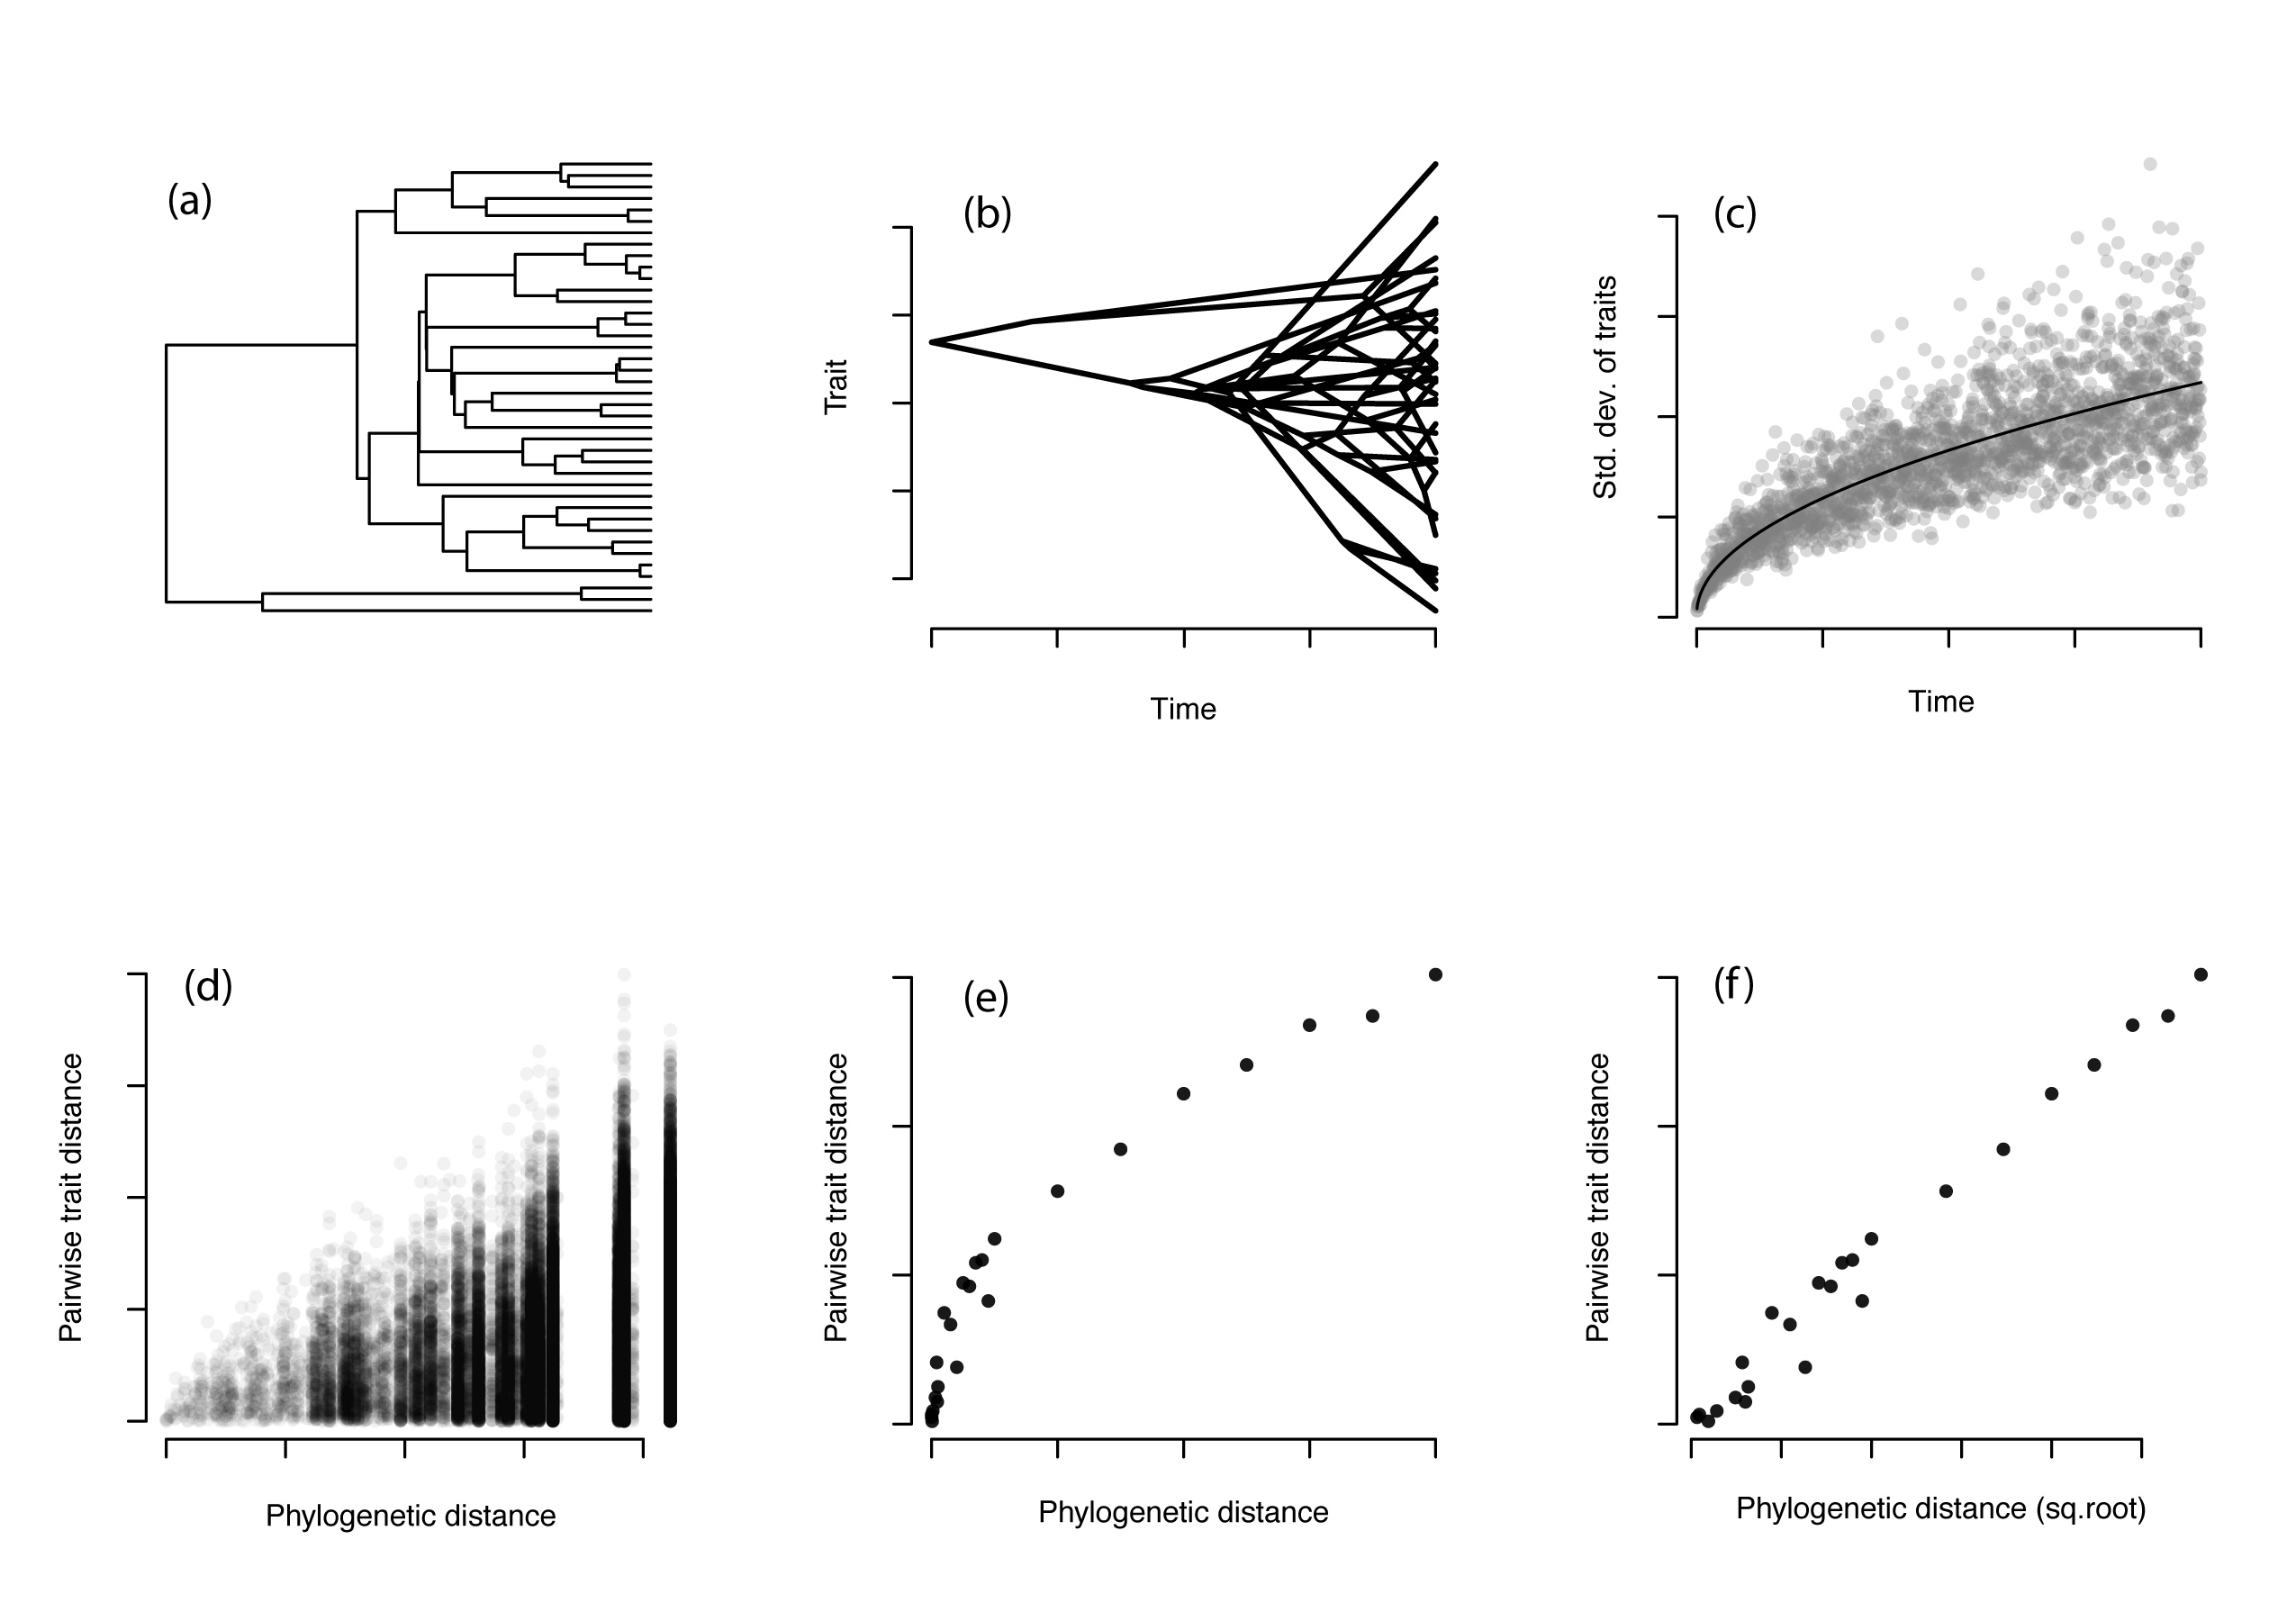
\includegraphics[width=1.00\textwidth]{sq_root_resub.png}
\caption{Panel (a) shows a Yule phylogeny. Panel (b) shows a ``traitgram'' with one Brownian motion 
simulation with the trait value on the y--axis.  Panel (c) shows the effect of time on the standard deviation of trait values at the tips for 2000 simulations with the same Brownian motion rate parameter; each point represents the standard deviation of the trait values of extant species within a separate simulation.  Panel (d) shows the pairwise trait differences for 50000 simulations plotted against phylogenetic distance.  Panel (e) simply takes the data from panel (d) and places them in bins, to show the statistical expectation at a given relatedness.  Panel (e) shows the effect of taking the square root of the phylogenetic distance matrix on the relationship between the phylogenetic distance and the expected trait difference.  Note that the expectation for the trait standard deviation and the pairwise difference is linear with respect to the square root of time as shown analytically in the text.  All simulations use code from FitzJohn (2012) and Revell (2012).}
\label{sq_root_fig}
\end{figure}

While this technical point is well understood in parts of the comparative methods literature 
\citep{Hardy2012}, the implications for many ecological applications has gone largely unnoticed. 
If evolutionary relatedness is used as a proxy for functional distance, the non-linearity of their 
scaling relationship means that more recent evolution should have a disproportional 
influence on contemporary ecology. Current methods used in community phylogenetics \citep[see 
review of methods 
in][]{vellend2010} typically treat evolutionary relatedness linearly; 1 and 6 million 
year relatedness difference is treated as having the same expected effect as a 
101 and 106 million year relatedness difference. All evolutionary time is 
considered equal, whether that time occurred over the last 5 million years or 
more than 100 million years ago. Combined with imbalanced trees, this creates 
a problem that is well known in empirical investigations: the statistical 
over-weighting of early-diverged, low diversity clades \citep{Kembel2006}. 
When those clades are included in the sample (or in a randomization), they 
have a disproportionate weight on the test statistic, a weight that is highly 
disproportionate to the expected trait difference under a Brownian model.  

The root of this problem is in the distribution of pairwise phylogenetic distances.  In the 
basic simulated birth-death trees, there is an equal probability at every time 
step for every branch of either a speciation or an extinction event.  This creates what are known as balanced trees \citep[][also Figure 
\ref{tree_fig}]{heard1997}. Balanced trees are rare in empirical studies, as heterogeneity in net diversification \citep{alfaro2009} creates trees that are imbalanced \citep{mooers1995} and have peculiar distributions of pairwise distances (e.g. the vascular plant tree from \citet{zanne2014} in Figure \ref{phylo_dist_hist}).  

\begin{figure}[H]
\centering
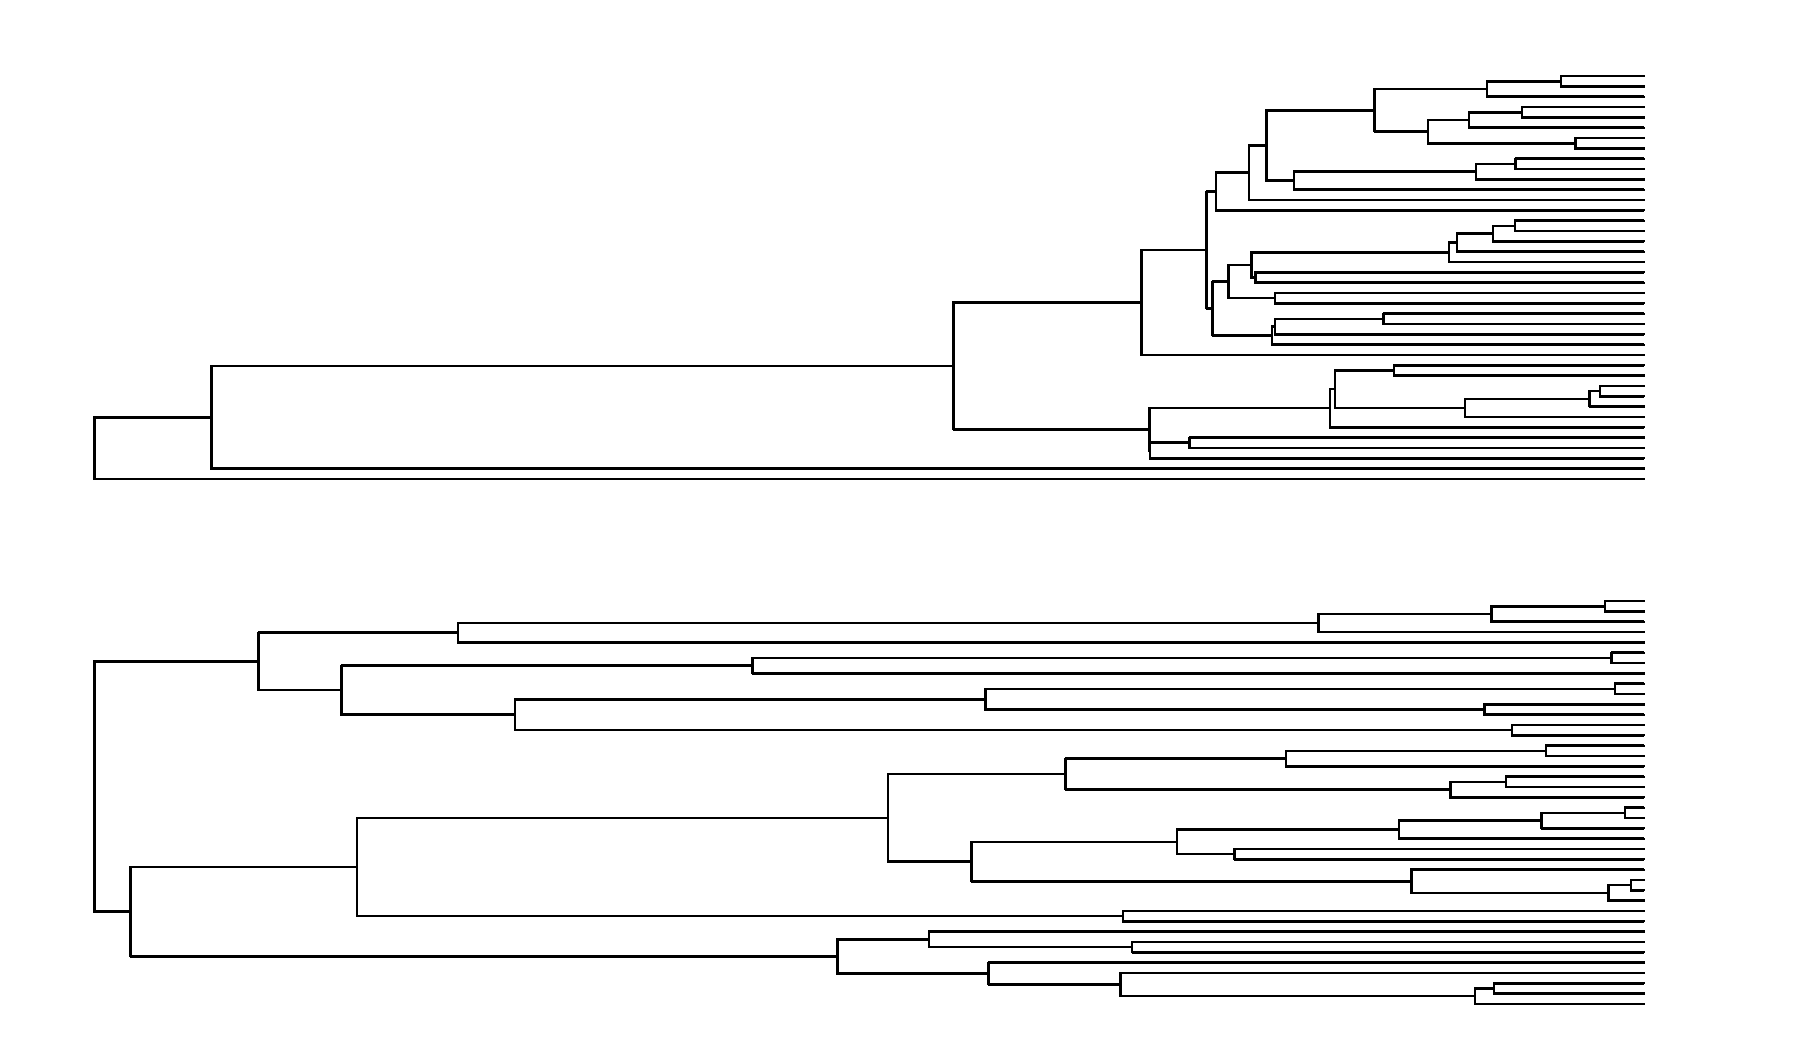
\includegraphics[width=1.00\textwidth]{trees_resub.pdf}
\caption{Example of a real tree (top), obtained by randomly selecting taxa from the Zanne et al. (2014) tree, compared with a 
homogeneous birth-death simulation tree (bottom).}
\label{tree_fig}
\end{figure}

Drawing from theory on Brownian motion reveals a simple solution to the weighting 
problem: a square--root transform of the phylogenetic distance matrix. For 
example, the mean pairwise distance \citep[sensu][]{Webb2000}:
\begin{equation} 
MPD=\frac{2\sum_{i=1}^{n-1} \sum^n_{j=i+1} d_{i,j}}{(n)(n-1)}
\end{equation} 
can be redefined as the mean of the square--root transformed pairwise distances:
\begin{equation} 
MPD^*=\frac{2\sum_{i=1}^{n-1} \sum^n_{j=i+1} \sqrt{d_{i,j}}}{(n)(n-1)}
\end{equation} 
where $n$ is the number of taxa and $d_{i,j}$ is the pairwise phylogenetic 
distance between species $i$ and species $j$. This quantity $MPD^*$ is 
proportional to the mean of the expected pairwise differences for traits 
evolving under a Brownian model, for both one trait in one dimension and for 
$m$ traits in $m$ dimensional space. This equation is provided as an example: 
very similar adjustments are possible to most of the common community 
phylogenetics statistics \citep[see definitions within][]{vellend2010}, simply 
via a square-root transform of the distance matrix.  

With this transformation, long--ago time is down weighted compared to recent 
time. As such, the effect of the presence or absence of a species on MPD
is weighted in proportion to the mean pairwise expected trait difference to all other species under a Brownian model. In practical terms this re-scaling can be accomplished exceedingly 
easily with one additional line of code in combination with the tools in 
widely available statistical packages
\citep{Kembel2010}. 

\begin{figure}[H]
\centering
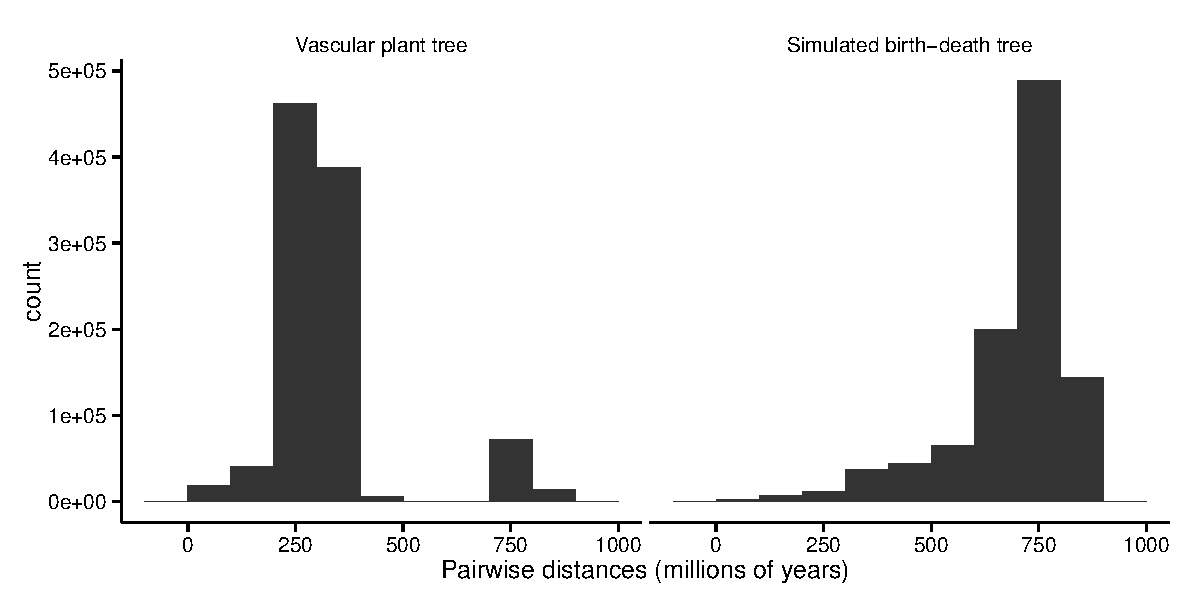
\includegraphics[width=1.00\textwidth]{phylo_dist_hist_corrected.pdf}
\caption{The pairwise phylogenetic distances from a recent phylogeny of vascular plants by Zanne et al. (2014) and a simulated phylogeny 
of the same age and number of
extant species.}
\label{phylo_dist_hist}
\end{figure} 

\section{Simulations}

To explore the empirical implications of this idea, we conducted simulations applying a similar framework to that described by \citet[][in this case repeating the `filtering-derived' and `neutral assembly' algorithms]{kraft2007}. We simulated trait evolution by Brownian motion on both a real tree and a homogenous birth-death simulated tree (Figure \ref{tree_fig}). To keep the pool size (number of tree tips) consistent across the real and simulated trees, the real tree was randomly pruned down to 200 taxa. In each run, we 'evolved' a trait across the phylogeny and then applied one of two community assembly filters to obtain a final community of 40 taxa. Under the 'filtering derived' assembly filter, the most derived (extreme) trait-value was treated as the optimum, with the remaining 39 places in the community selected from taxa having the nearest trait values to that optimum. This process simulated  community assembly via habitat filtering \citep{Diaz1998}, whereby the abiotic environment sets some threshold on the range of strategies (and thereby trait values) that are able to sustain a positive population growth rate (e.g. tolerance of inundation along a hydrological gradient). In contrast with the deterministic nature of the `filtering-derived' algorithm, under the `neutral assembly' algorithm the community was obtained by randomly selecting 40 species independent of their trait values. One--thousand runs were conducted for each community assembly algorithm on each of the real and simulated phylogenies. Finally, we quantified the effect of the filter using conventional community phylogenetics methods (MPD and MNTD - mean nearest taxon distance), and compared the standard approach with that of a square--root transform of the phylogenetic distance matrix (all code to perform replicate simulations is provided in Appendix B). 

Simulation results indicate the transformed test has considerably higher statistical power (Figure 
\ref{stat_power_fig}) for detecting the signal of community assembly. Using 
the square--root transform improved 92\% of trials for both MPD and MNTD. Using the standardized effect size metric developed by 
\cite{Webb2000}, whereby:

$$SES_{METRIC} = \frac{METRIC_{observed} - mean(METRIC_{null})}{sd(METRIC_{null})}$$

the median improvement in standardized effect size was 0.64 
for MPD and 0.43 for MNTD (simulated and real trees combined). 
This is a comparatively large increase in effect size from a simple statistical 
adjustment.  The improvement was similar for real and simulated 
trees, but may be more crucial in the real case because the general power of 
community phylogenetics is lower for the real tree \citep{Kembel2006}. While a comprehensive exploration of the effect of the transformation on type 1 error rates is beyond the scope of this paper  \citep[see][]{kraft2007}, simulations indicated that the expected reduction in type 2 error rate is in the order of 5-25\% (depending on the community to pool size ratio and other factors).

\begin{figure}[H]
\centering
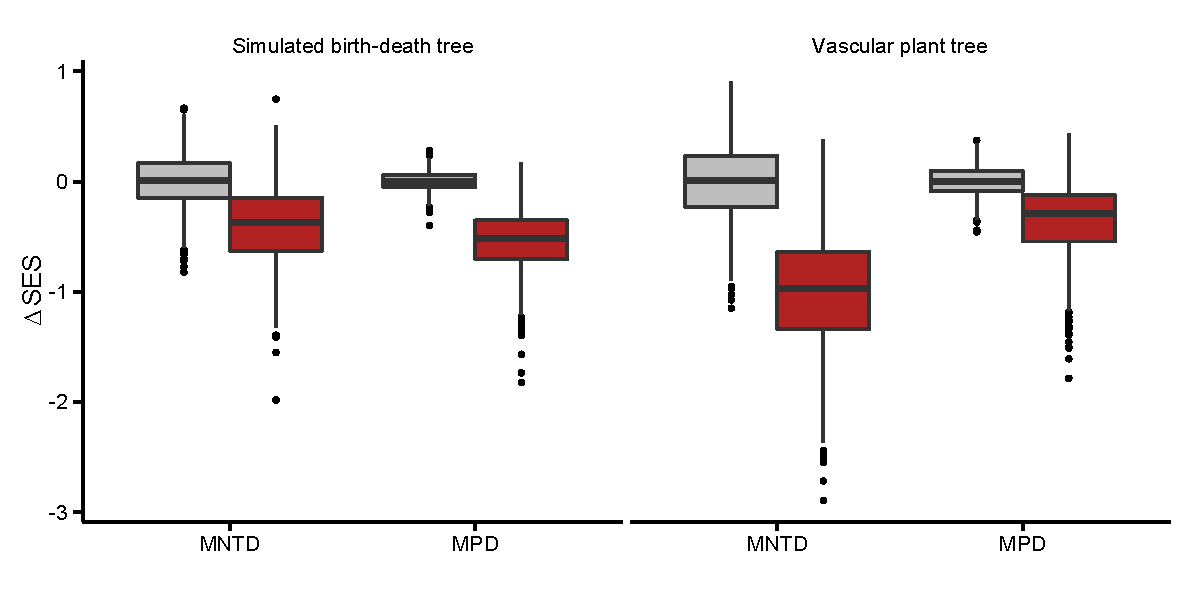
\includegraphics[width=1.00\textwidth]{bm_diff_p220_c40.pdf}
\caption{Improved statistical power from down-weighting long-ago evolution: change in standardized effect size for mean pairwise 
distance (MPD) and mean nearest taxa distance (MNTD) using a square-root transformed phylogenetic distance matrix versus the 
conventional approach. Box plots with grey-fill group communities assembled under a neutral (random sample) model; box plots with 
red-fill group communities assembled under a 'habitat filter' model.}
\label{stat_power_fig}
\end{figure}

 
\section{Other models of trait evolution}

While a highly useful ``default'' model, we do not expect that a Brownian 
motion model will prove to be a fully adequate model for trait 
evolution at large scales. In general, the current evidence suggests that 
actually the square--root transform does not go far enough toward 
down--weighting long--ago evolution compared to recent evolution in many cases 
\citep{butler2004, harmon2010, smith2010evolution}. In the event that there 
are bounding or mean-reverting processes \citep[e.g. Ornstein--Uhlenbeck (OU)][]{butler2004}, phylogenetic 
signal will be less strong than under a Brownian model.  Under these alternative models the effect 
of evolutionary 
relatedness
decays more rapidly, a phenomena defined as ``phylogenetic half-life'' by \citet{hansen2008comparative}.  
If trait evolution typically includes this type of process, the problem we describe here will be even more extreme. 
In this case \citep[see][]{kelly2014phylogenetic}, the square--root transformation will not 
go far enough. For the alternatives to Brownian motion, such as OU and
heterogeneous models where rates of evolution vary among clades \citep{beaulieu2012modeling}, there are analogous tree scaling approaches \citep{Pearse2013a}, but these, unlike the square--root transformation, 
require \emph{a priori} information about trait evolution in the relevant 
clade.  

\section{Conclusion}

We recommend a square--root transform of the phylogenetic distance matrix for 
all uses where phylogenetic relatedness is used as a proxy for current--day 
functional disparity. There are some cases where the number of years of 
evolutionary history in a place may be an interesting quantity in and of 
itself \citep{purvis2000}. In those cases linear relatedness may still be of 
interest; however, many ecological studies use evolutionary relatedness as a 
proxy for trait dissimilarity and in these cases using relatedness linearly 
will decrease the power of the investigation. 

While we have made a statistical argument above, in conclusion we stress that 
this is actually a conceptual point. We argue that conventional approaches over-weight long-ago 
evolutionary time and under-weight recent evolution both conceptually and statistically, and in 
doing so inadvertently limit the statistical power and success of efforts to leverage phylogenetic 
information in ecological contexts. There are many other reasons why the mapping of 
ecological process to phylogenetic community patterns may be inconclusive \citep{Mayfield2010, Godoy2014}; many of these issues are hard to address.  Here, we have identified one problem---
the weighting of evolutionary history---where a simple 
adjustment may help.

Of course, by using the square-root transformation we make the assumption that trait differences scale linearly with ecological fitness. While disentangling the ecological/evolutionary processes is somewhat intractable in this instance, this is at least a parsimonious assumption. Instead, justification for using more complex measures of functional distance (e.g. squared distance) in the context of ecological selection/assembly should be contingent on supporting theory. To our knowledge none exists. The magnitude of fitness-trait relationships has received some attention \citep{Kimball2011, Adler2013a} but explicitly exploring their scaling properties could well prove an invaluable area of future research.

In general, there needs to be a more nuanced use of evolutionary relatedness within community 
ecology.  By improving the connection between metrics within community phylogenetics and trait 
evolution, we can increase the power and utility of using evolutionary relatedness to ask ecological questions. 
This methodological update will not be a one-off: as our understanding of the processes and patterns in trait macro-evolution at large 
scales grows \citep{omeara2012, pennell2013integrative}, the phylogenetic metrics used in contemporary ecology will need to be 
continually updated.

\subsection*{Acknowledgements}

Thanks to Nathan Kraft, Rich FitzJohn, Rob Kooyman, Sandrine Pavoine and an anonymous reviewer for insightful comments.  

\subsection*{Data accessibility}

R code to reproduce simulations provided in Appendix B.

\nocite{zanne2014, FitzJohn2012, Revell2012}
%\bibliographystyle{mee}
%\bibliography{bm_scaling}


